% questions.tex —— 1977 年·江苏常州市初试卷 · 题目内容片段（无答案）
% 由 tools/generate_projects.py 依来源总账自 1977/1977_数学真题_江苏常州市初试_试题.md 生成，勿手改（改源 MD 后重跑）


\gkpart{数学试卷（江苏常州市初试卷）}

\begin{gktip}
\textbf{来源说明}：本题面依据固定源 PDF《1977江苏常州市初试》共 3 页逐题转录。原卷系 1977 年江苏省常州市高考初试（预选）数学卷，收于初试题汇编，页首标题排作「二、常州市」（汇编第二部分），本文 H1 按原卷逐字保留，H2 为编者所加。原卷题号已为阿拉伯数字「N．」并逐题标注分值（7、7、6 分与十个 8 分，合计 100 分），本文照录。原卷为纯题面卷，未附答案；配套答案与解析为本库编者独立推导，\textbf{非官方标准答案}。扫描件第 2 页左下印有书籍页码 232，本文按 PDF 页序记录。
\end{gktip}

\par\medskip

\begin{question}
\gkti{1}\textbf{（7 分）} 计算：

\nopagebreak[4]
\[
-1-\left(-5\frac{1}{2}\right)\times\frac{4}{11}+(-2)^3\div\left[(-3)^2+7\right].
\]

\end{question}
\begin{question}
\gkti{2}\textbf{（7 分）} 计算：

\nopagebreak[4]
\[
\frac{2}{2+\sqrt{2}}+\frac{1}{\sqrt{3}-\sqrt{2}}-\frac{3+\sqrt{3}}{3-\sqrt{3}}.
\]

\end{question}
\begin{question}
\gkti{3}\textbf{（6 分）} 计算：$\log_2(1+\lg10)$。

\end{question}
\begin{question}
\gkti{4}\textbf{（8 分）} $\sin390^\circ\cos(-60^\circ)+\sin120^\circ\cos750^\circ.$

\end{question}
\begin{question}
\gkti{5}\textbf{（8 分）} 化简：$a+\sqrt{a^2-2a+1}$。

\end{question}
\begin{question}
\gkti{6}\textbf{（8 分）} 已知 $a=9$，$b=\sqrt{3}$，求

\nopagebreak[4]
\[
a^{\frac{3}{2}}b\left(\frac{b^2}{a}\right)^{\frac{1}{2}}\div\left(\frac{1}{a}\right)^{-\frac{1}{2}}
\]

的值。

\end{question}
\begin{question}
\gkti{7}\textbf{（8 分）} 求函数 $y=\sqrt{x-3}+\sqrt{5-x}$ 的自变量的取值范围。

\end{question}
\begin{question}
\gkti{8}\textbf{（8 分）} 求证：

\nopagebreak[4]
\[
\operatorname{ctg}\frac{\pi}{8}-\operatorname{tg}\frac{\pi}{8}=2.
\]

\Needspace{0.4\textheight}
\end{question}
\begin{question}
\gkti{9}\textbf{（8 分）} 要建造轮廓为矩形的猪舍四间，按实线部分砌墙，若墙的总长为 $32$ 米，问每间猪舍的长、宽为几米时面积最大？每间猪舍的最大面积是多少？
\nopagebreak[4]
\begin{center}% 1977 年江苏常州市初试卷第 9 题：四间猪舍砌墙示意——上边与五条竖墙为实线（砌墙），
% 下边为虚线（沿原有墙不砌）（按源卷第 2 页布局）
\begin{tikzpicture}[scale=0.8]
  \draw[thick] (0,3)--(12,3);
  \draw[dashed] (0,0)--(12,0);
  \foreach \x in {0,3,6,9,12}{\draw[thick] (\x,0)--(\x,3);}
\end{tikzpicture}
\end{center}
\nopagebreak[4]
\Needspace{0.4\textheight}
\end{question}
\begin{question}
\gkti{10}\textbf{（8 分）} 如图：割线 $PO$ 交 $\odot O$ 于 $C$、$D$，割线 $PA$ 交 $\odot O$ 于 $A$、$B$，
\nopagebreak[4]
\begin{center}% 1977 年江苏常州市初试卷第 10 题：圆 O 与两条割线——过圆心的割线 P-D-O-C，
% 圆外一点 P 的割线 P-B-A（按源卷第 2 页布局）
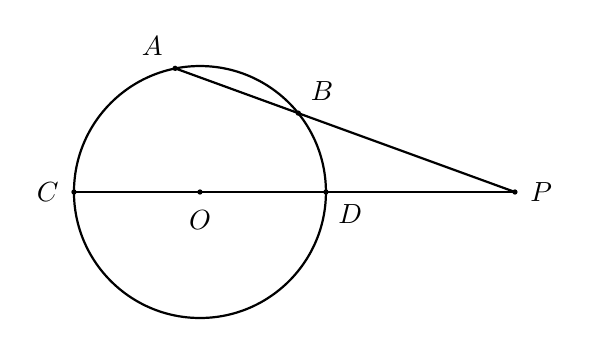
\begin{tikzpicture}[scale=0.8]
  \coordinate (O) at (0,0);
  \coordinate (P) at (5,0);
  \coordinate (C) at (-2,0);
  \coordinate (D) at (2,0);
  \coordinate (B) at (1.561,1.252);
  \coordinate (A) at (-0.394,1.963);
  \draw[thick] (0,0) circle (2);
  \draw[thick] (C)--(P);
  \draw[thick] (P)--(A);
  \fill (O) circle (1.2pt) node[below=3pt] {$O$};
  \fill (P) circle (1.2pt) node[right=2pt] {$P$};
  \fill (C) circle (1.2pt) node[left=2pt] {$C$};
  \fill (D) circle (1.2pt) node[below right=1pt] {$D$};
  \fill (B) circle (1.2pt) node[above right=1pt] {$B$};
  \fill (A) circle (1.2pt) node[above left=1pt] {$A$};
\end{tikzpicture}
\end{center}
\nopagebreak[4]
（1） 试证：$PA\cdot PB=PC\cdot PD$；

（2） 已知：$\odot O$ 的半径为 $1$，$PO=2$，$AB=1$，求 $PA$ 的长。

\Needspace{0.4\textheight}
\end{question}
\begin{question}
\gkti{11}\textbf{（8 分）} 右图是某物体的二视图，按 $1:1$ 的比例画出这个物体的直观图，并计算它的侧面积。
\nopagebreak[4]
\begin{center}% 1977 年江苏常州市初试卷第 11 题：物体二视图——正视图（底 24 高 16 的三角形）在上，
% 俯视图（24x24 带对角线的正方形）在下，含中心线与尺寸标注（按源卷第 2 页布局）
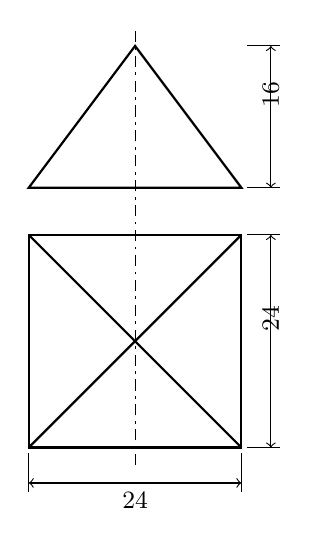
\begin{tikzpicture}[scale=0.75, font=\small]
  % 正视图：三角形
  \draw[thick] (-1.8,2.4)--(1.8,2.4)--(0,4.8)--cycle;
  % 俯视图：正方形与对角线
  \draw[thick] (-1.8,1.6)--(1.8,1.6)--(1.8,-2.0)--(-1.8,-2.0)--cycle;
  \draw[thick] (-1.8,1.6)--(1.8,-2.0);
  \draw[thick] (1.8,1.6)--(-1.8,-2.0);
  % 中心线（点划线）
  \draw[dash pattern=on 4pt off 2pt on 1pt off 2pt] (0,-2.3)--(0,5.1);
  % 尺寸标注引出线
  \draw[thin] (1.9,2.4)--(2.45,2.4);
  \draw[thin] (1.9,4.8)--(2.45,4.8);
  \draw[thin] (1.9,1.6)--(2.45,1.6);
  \draw[thin] (1.9,-2.0)--(2.45,-2.0);
  \draw[thin] (-1.8,-2.1)--(-1.8,-2.75);
  \draw[thin] (1.8,-2.1)--(1.8,-2.75);
  % 尺寸：16（正视图高）
  \draw[<->] (2.3,2.4)--(2.3,4.8) node[midway, right, rotate=90] {$16$};
  % 尺寸：24（俯视图宽）
  \draw[<->] (2.3,-2.0)--(2.3,1.6) node[midway, right, rotate=90] {$24$};
  % 尺寸：24（俯视图长）
  \draw[<->] (-1.8,-2.6)--(1.8,-2.6) node[midway, below] {$24$};
\end{tikzpicture}
\end{center}
\nopagebreak[4]
\end{question}
\begin{question}
\gkti{12}\textbf{（8 分）} 已知：三点 $A(-2,\ 9)$，$B(4,\ -4)$，$C(10,\ 8)$．试求：

（1） 过 $A$ 点且垂直于 $BC$ 的直线方程；

（2） $A$ 点到 $BC$ 的距离。

\Needspace{0.4\textheight}
\end{question}
\begin{question}
\gkti{13}\textbf{（8 分）} 如图：在直角坐标系中，$OA_0=1$，以 $OA_0$ 为一条直角边画出第一个直角三角形 $OA_0A_1$，又以 $OA_1$ 为一直角边画出第二个直角三角形 $OA_1A_2$，再以 $OA_2$ 为一直角边画出第三个直角三角形 $OA_2A_3$，依次继续画下去，试求：
\nopagebreak[4]
\begin{center}% 1977 年江苏常州市初试卷第 13 题：极坐标系中依次旋转 30 度的螺旋直角三角形序列
% OA0A1...A4（Ak 在极角 30k 度的射线上，直角顶点为 Ak），十二 条 30 度间隔射线按原卷标注（按源卷第 3 页布局）
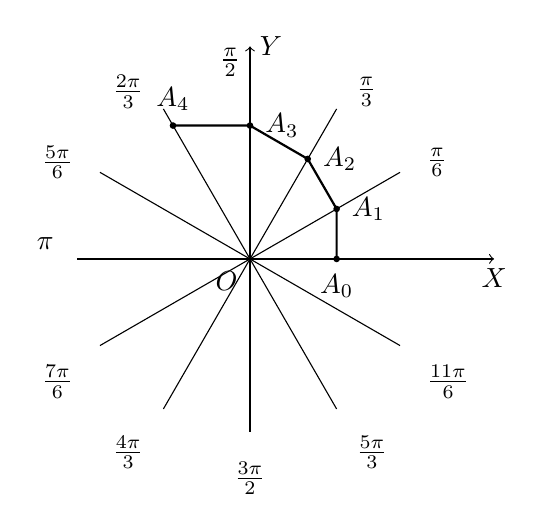
\begin{tikzpicture}[scale=1.0]
  % 十二条 30 度间隔射线
  \foreach \a in {0,30,...,330}{\draw[thin] (0,0)--(\a:2.2);}
  % 坐标轴
  \draw[->, thin] (0,0)--(3.1,0) node[below] {$X$};
  \draw[->, thin] (0,0)--(0,2.7) node[right] {$Y$};
  % 螺旋折线 A0-A1-A2-A3-A4（OA0=1 对应 1.1cm，公比 2/\sqrt{3}）
  \draw[thick] (1.1,0)--(1.1,0.635)--(0.733,1.270)--(0,1.694)--(-0.978,1.694);
  \fill (1.1,0) circle (1.2pt) node[below=2pt] {$A_0$};
  \fill (1.1,0.635) circle (1.2pt) node[right=2pt] {$A_1$};
  \fill (0.733,1.270) circle (1.2pt) node[right=2pt] {$A_2$};
  \fill (0,1.694) circle (1.2pt) node[right=2pt] {$A_3$};
  \fill (-0.978,1.694) circle (1.2pt) node[above=2pt] {$A_4$};
  \node[below left=1pt] at (0,0) {$O$};
  % 射线极角标注
  \node[right] at (30:2.45) {$\frac{\pi}{6}$};
  \node[right] at (60:2.45) {$\frac{\pi}{3}$};
  \node[left] at (90:2.5) {$\frac{\pi}{2}$};
  \node[left] at (120:2.45) {$\frac{2\pi}{3}$};
  \node[left] at (150:2.45) {$\frac{5\pi}{6}$};
  \node[above] at (180:2.6) {$\pi$};
  \node[below left] at (210:2.45) {$\frac{7\pi}{6}$};
  \node[below left] at (240:2.45) {$\frac{4\pi}{3}$};
  \node[below] at (270:2.45) {$\frac{3\pi}{2}$};
  \node[below right] at (300:2.45) {$\frac{5\pi}{3}$};
  \node[below right] at (330:2.45) {$\frac{11\pi}{6}$};
\end{tikzpicture}
\end{center}
\nopagebreak[4]
（1） $A_6$ 点的极坐标；

（2） 第十二个直角三角形的面积（精确到 $0.01$）。

已知 $\lg2=0.3010$，$\lg3=0.4771$。原卷随题印有「反对数表」节选（标准四位反对数表第 80—84 行、第 0—5 列），转录如下：

\begin{center}
\begin{tabular}{lllllll}
\toprule
m & 0 & 1 & 2 & 3 & 4 & 5 \\
\midrule
80 & 6310 & 6324 & 6339 & 6353 & 6368 & 6383 \\
81 & 6457 & 6471 & 6486 & 6501 & 6516 & 6531 \\
82 & 6607 & 6622 & 6637 & 6653 & 6668 & 6683 \\
83 & 6761 & 6776 & 6792 & 6808 & 6823 & 6839 \\
84 & 6918 & 6934 & 6950 & 6966 & 6982 & 6998 \\
\bottomrule
\end{tabular}
\end{center}

\end{question}